\section{Summary}
	\begin{align}
		x = \ &\text{position}& \notag \\
		\Delta x = \ &\text{displacement}& \notag \\
		= \ &x_{f} - x_{i}& \notag \\
		\bar{v} = \ &\text{average velocity}& \notag \\
		= \ &\frac{\Delta x}{\Delta t}& \notag \\
		v = \ &\text{instantaneous velocity}& \notag \\
		= \ &\frac{dx}{dt} = \text{slope of x vs. t}& \notag \\
		\text{Avg Speed} = \ &\frac{\text{distance traveled}}{\text{time elapsed}}& \notag
	\end{align}

\section{Acceleration}

	\begin{align}
		&\text{Let} \ & &\bar{a} = \ & &\text{average acceleration}& \notag \\
		&& &\bar{a} \equiv \ & &\frac{\Delta v}{\Delta t} = \frac{v_{f} - v_{i}}{\Delta t} = \frac{\text{change in velocity}}{\text{time elapsed}}& \notag
	\end{align}

	Example: A car goes from $20 \ mph$ to $60 \ mph$ in $8 \ s$. What is its average acceleration?

	\begin{align}
		v_{i} = \ &20 \ mi/h& \notag \\
		v_{f} = \ &60 \ mi/h& \notag \\
		\Delta t = \ &8 \ s& \notag \\
		\bar{a} = \ &\frac{\Delta v}{\Delta t} = \frac{v_{f} - v_{i}}{\Delta t}& \notag \\
		= \ &\frac{60 \ mi/h - 20 \ mi/h}{8 \ s}& \notag \\
		= \ &\frac{40 \ mi/h}{8 \ s}& \notag \\
		= \ &5 \ \frac{mi}{h \times s}& \notag
	\end{align}

	Example: Justin Bieber's Limo goes from $30 \ m/s$ to a stop in $0.10 \ s$. What is its average acceleration?

	\begin{align}
		v_{i} = \ &30 \ m/s& \notag \\
		v_{f} = \ &0 \ m/s& \notag \\
		\Delta t = \ &0.10 \ s& \notag \\
		\bar{a} = \ &\frac{\Delta v}{\Delta t} = \frac{v_{f} - v_{i}}{\Delta t}& \notag \\
		= \ &\frac{0 \ m/s - 30 \ m/s}{0.10 \ s}& \notag \\
		= \ &\frac{- 30 \ m/s}{0.10 \ s}& \notag \\
		= \ &- 300 \ \frac{m/s}{s} = - 300 m/s^{2}& \notag
	\end{align}
	($-$ means slowing) \newline

	Let
	\begin{align}
		a = \ &\text{instantaneous acceleration}& \notag \\
		= \ &lim_{\Delta t \to 0} \frac{\Delta v}{\Delta t}& \notag \\
		a \equiv \ &\frac{dv}{dt} = \text{rate of change of velocity}& \notag \\
		= \ &\text{slope of tangent line to v vs. t}& \notag
	\end{align}

	Example:

	\begin{align}
		x = \ &3 \ m + \left( 17 \ m/s \right)t + \left(7 \ m/s^{3} \right)t^{3}& \notag \\
		Find: \ &\text{a) velocity at }3 \ s& \notag \\
		&\text{b) velocity at }5 \ s& \notag \\
		&\text{c) average acceleration from }3 \ s \to 5 \ s& \notag \\
		&\text{c) instantaneous acceleration at }4 \ s& \notag
	\end{align}
	a)
	\begin{align}
		v = \ &\frac{dx}{dt} = 17 \ m/s + \left( 21 \ m/s^{3} \right)t^{2}& \notag \\
		v(3 \ s) = \ &17 \ m/s + \left( 21 \ m/s^{3} \right)(3 \ s)^{2}& \notag \\
		= \ &17 \ m/s + 189 \ m/s& \notag \\
		= \ &206 \ m/s& \notag
	\end{align}
	b)
	\begin{align}
		v(5 \ s) = \ &17 \ m/s + \left( 21 \ m/s^{3} \right)(5 \ s)^{2}& \notag \\
		= \ &17 \ m/s + 525 \ m/s& \notag \\
		= \ &542 \ m/s& \notag
	\end{align}
	c)
	\begin{align}
		\bar{a} = \ &\frac{\Delta v}{\Delta t} = \frac{v_{f} - v_{i}}{\Delta t} = \frac{542 \ m/s - 206 \ m/s}{5 \ s - 3 \ s}& \notag \\
		= \ &\frac{336 \ m/s}{2 \ s} = 168 \ m/s^{2}& \notag
	\end{align}
	d)
	\begin{align}
		a = \ &\frac{dv}{dt}& \notag \\
		= \ &\frac{d}{dt}\left[ 17 \ m/s + (21 \ m/s^{3})t^{2} \right]& \notag \\
		= \ &0 + (42 \ m/s^{3})t& \notag \\
		a(4 \ s) = \ &(42 \ m/s^{3})(4 \ s)& \notag \\
		= \ &168 \ m/s^{2}& \notag
	\end{align}
	\begin{figure}[H]
		\begin{center}
			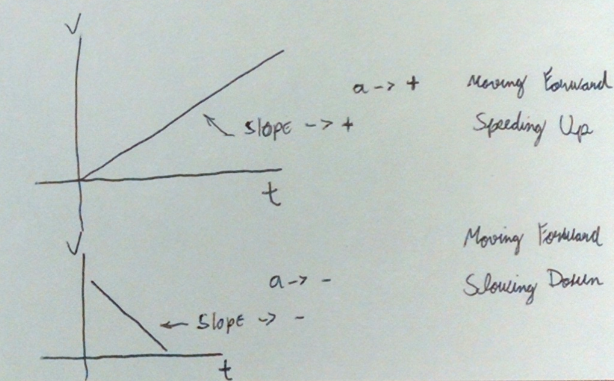
\includegraphics[scale=0.43]{01_27_01}
			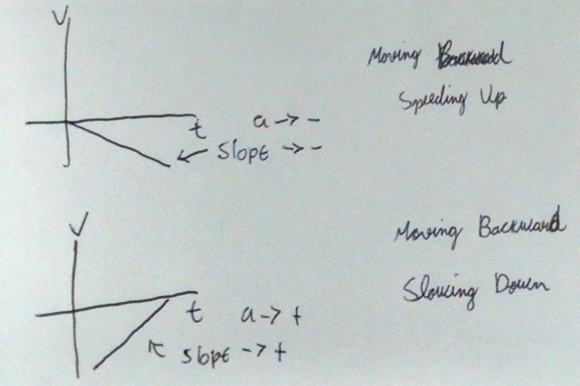
\includegraphics[scale=0.43]{01_27_02}
			\caption{Graphics of Acceleration}
			\label{fig:01_27_01-02}
		\end{center}
	\end{figure}

	\begin{align}
		&t_{i}& &\to& &0& \notag \\
		&t_{f}& &\to& &t& \notag \\
		&x_{i}& &\to& &x_{0}& \notag \\
		&x_{f}& &\to& &x& \notag \\
		&v_{i}& &\to& &v_{0}& \notag \\
		&v_{f}& &\to& &v& \notag
	\end{align}

	Suppose $a = $ constant

	\begin{align}
		\bar{a} = \ &a& \notag \\
		\frac{v - v_{0}}{t} = \ &a& \notag \\
		v - v_{0} = \ &at& \notag \\
		v = \ &v_{0} + at \text{ : }v(t)& \\
		x = \ &x_{0} + v_{0}t + \frac{1}{2} at^{2} \text{ : }x(t)& \\
		x = \ &x_{0} + \frac{1}{2} (v_{0} + v)t \text{ : no }a& \\
		2a(x - x_{0}) = \ &v^{2} - v_{0}^{2} \text{ : no }t&
	\end{align}
